\chapter{Conclusion \& Future Work}

\section{Conclusion}

\begin{figure}[ht!]
    \centering
    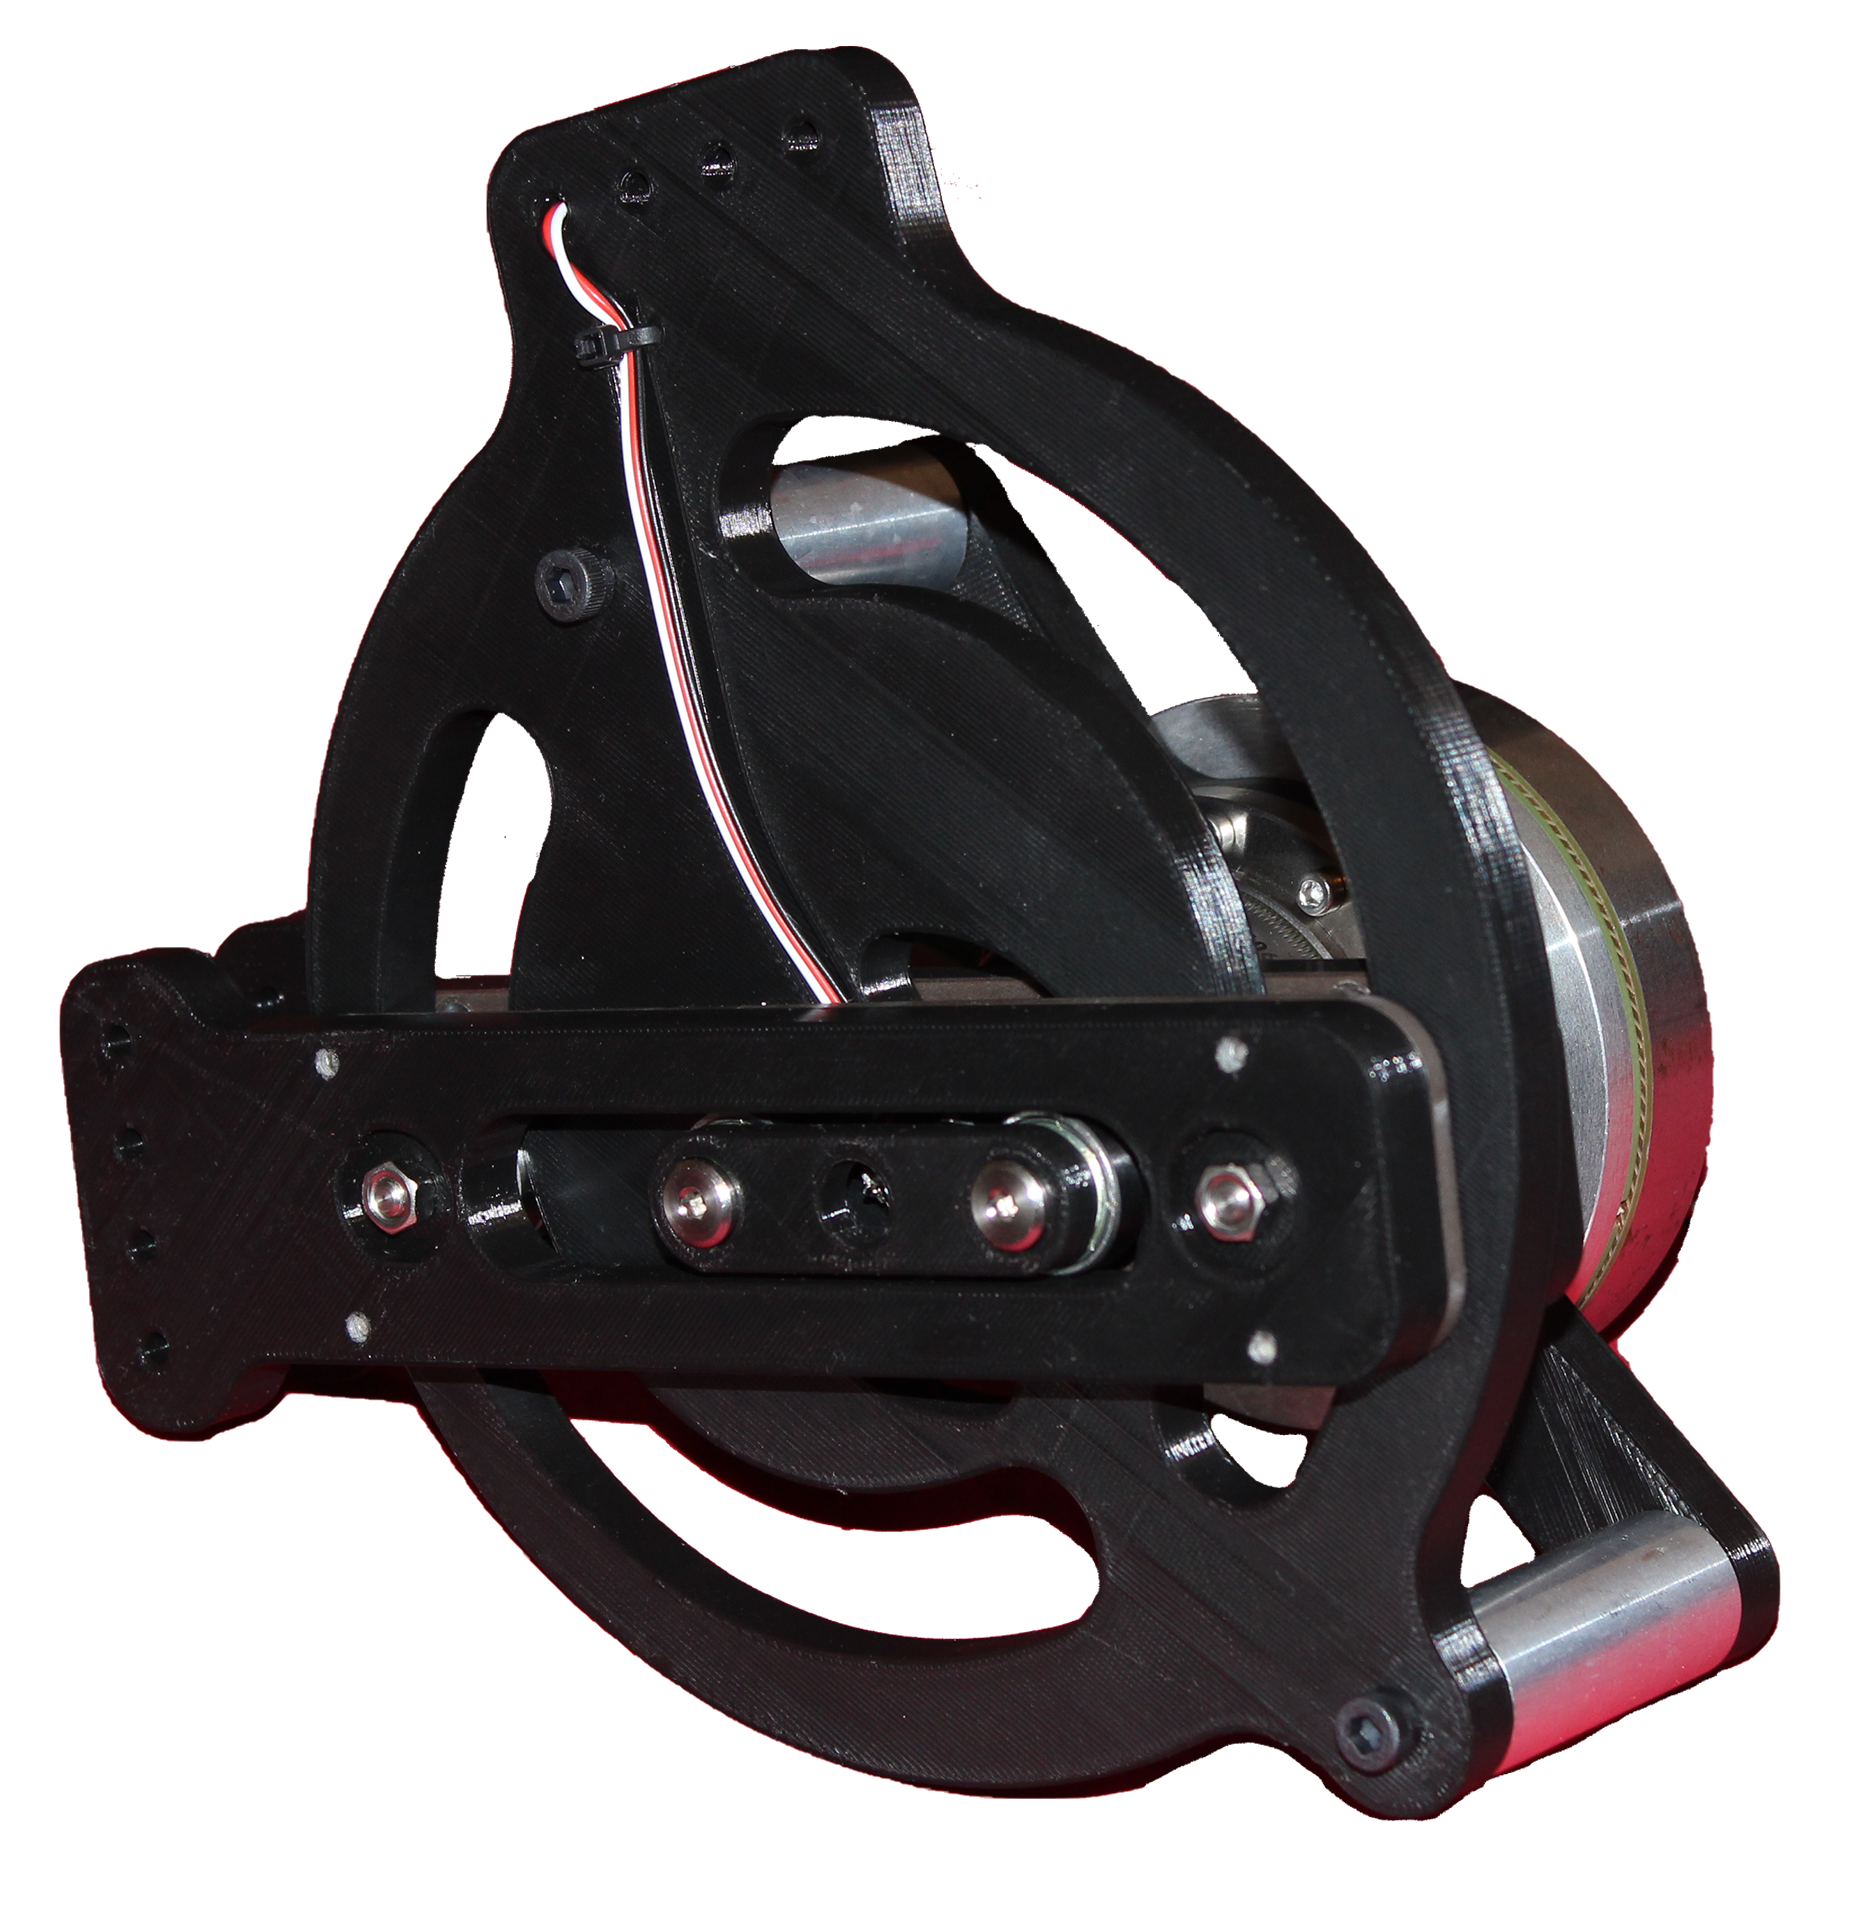
\includegraphics[width=0.7\linewidth]{Figures/KneeJointPrototype_ClearBackground.png}
    \caption{A picture of a left-sided knee joint prototype manufactured as a part of this thesis}
    \label{fig:KneeJointPicture}
\end{figure}

The proposed knee joint developed and tested in this thesis succeeded in all design requirements, even exceeding them in some scenarios. Experimentation showed that the knee could follow a defined tibiofemoral joint trajectory within \(1mm\) of accuracy. The joint itself can also be easily customized to each patient, with only one custom part needing to be manufactured per person per joint. Integrated sensors allow it to sense joint position and report it to the WPI LARRE hardware controllers. Strength analysis demonstrated that the joint can be manufactured from either PLA plastics using a conventional FDM 3D printer or machined out of aluminum. The joint will be able to support the stresses that come from common rehabilitation exercises including sit/stand exercises and walking gait exercises. Finally, the joint will be able to be integrated in the WPI LARRE (Legged Articulated Robotic Rehabilitation Exoskeleton). However, the design proposed is not limited to exoskeletons; the concept of using a cam mechanism to match tibiofemoral relationships can be applied to other orthoses that need to be powered.

\begin{figure}[ht!]
    \centering
    % \missingfigure[]{Picture of Knee Joint}
    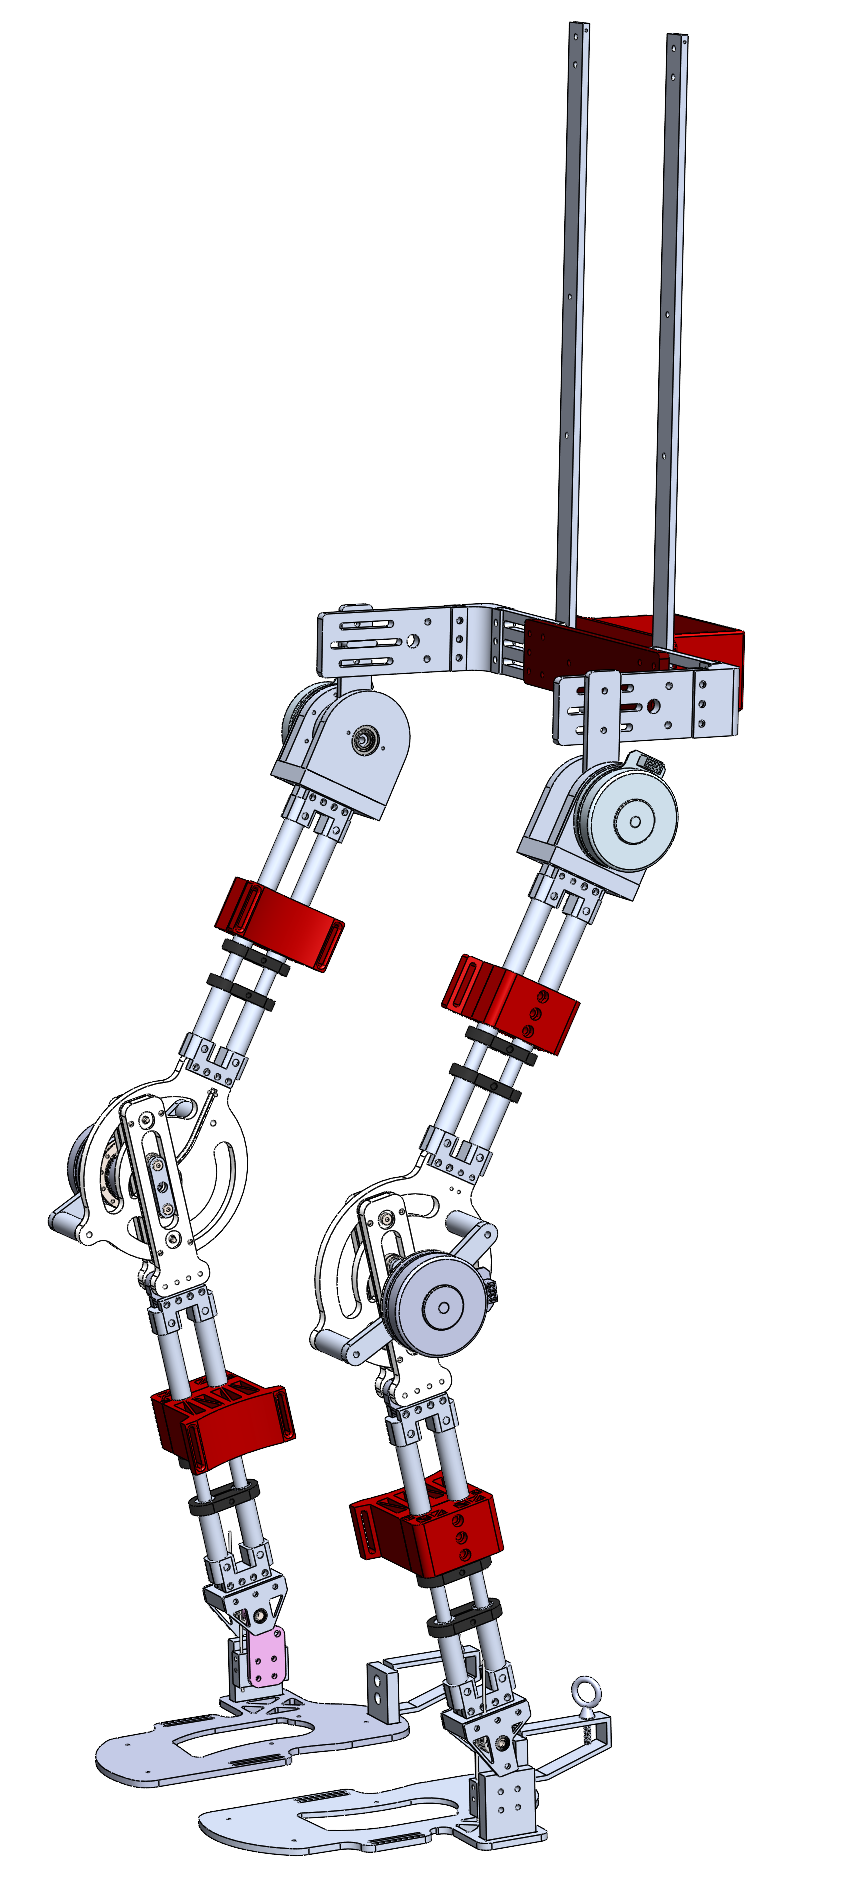
\includegraphics[width=0.4\linewidth]{Figures/FinalExoRender.png}
    \caption{Proposed knee joint mounted to a model of WPI LARRE}
    \label{fig:KneeOnExo}
\end{figure}

% TODO: Add conclusion for the knee parameterization

\section{Future Work}

While the design was able to match and even exceed the design requirements, more research is needed. From a design perspective, the joint can be made much smaller than the existing design. The motor and gearbox can be integrated in the joint to offer a lower profile exterior. Additionally, a more efficient and less expensive no-backlash gearbox such as a cycloidal gearbox can be integrated to replace the {Harmonic\texttrademark} gearbox used in this study. 

Additionally, more research is needed in knee movement in an exoskeleton. The research discussed in \autoref{sec:KneeModel} demonstrates the relationship between the tibia and femur, and does not look how skin movement changes the trajectory. Studies using the parameterization method discussed in \autoref{sec:KneeParams} may demonstrate a more accurate relationship to be used with this knee joint, as well as determine the parameters of a patient's knee. This would create a future where a lower-limb paralysis patient would be able to receive a perfectly personalized knee joint for their rehabilitation exoskeleton using an imaging system.